\section{Resultados y Discusión}

\subsection{Experimento 1: Método de la potencia}

En primer lugar vemos cuantas iteraciones demandó cada $\alpha$ para llegar a un autovalor con una diferencia con respecto al autovalor anterior menor a épsilon. \\

\begin{figure}[H]
     \begin{center}
     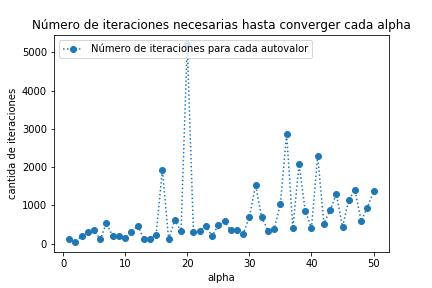
\includegraphics[width=100mm]{img/iteraciones_x_alpha.png} 
    \end{center}
\caption{Iteraciones por cada $\alpha$} \label{fig:exp1-iters}
\end{figure}

Exceptuando el máximo de 5204 iteraciones para uno de los $\alpha$, la mayoría no pasa las cientos de iteraciones hasta converger hacia lo que nosotros definimos como convergencia ($\epsilon$ < $10^{-9}$). 
El promedio es de 739 iteraciones con una mediana de 420.

Tomando solo el caso del $\alpha$ que más tarda en converger, graficamos el $\epsilon$ para cada iteración.\\

\begin{figure}[H]
     \begin{center}
     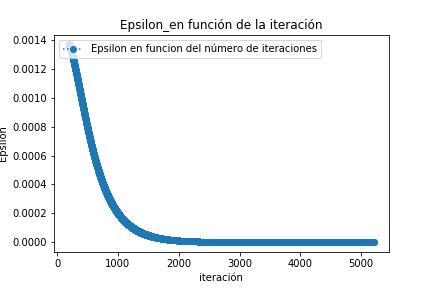
\includegraphics[width=100mm]{img/epsilon_x_iter.png} 
    \end{center}
\caption{Epsilon por iteración} \label{fig:exp1-epsilon}
\end{figure}

Vemos que este va convergiendo conforme avanza el número de iteraciones. Los otros $\alpha$ muestran una curva similar pero obviamente con un corte menor. \\

\begin{figure}[H]
     \begin{center}
     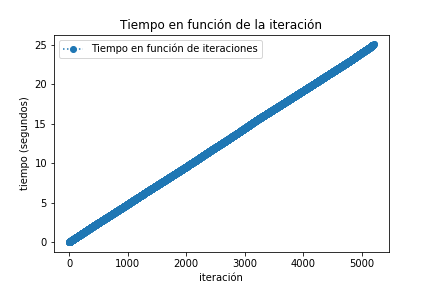
\includegraphics[width=100mm]{img/tiempo_x_iter.png} 
    \end{center}
\caption{Tiempo por iteración} \label{fig:exp1-tiempo}
\end{figure}

Arriba se observa cómo se acumula el tiempo a medida que iteramos. Considerando que la mediana es de 420 y el promedio es de 739 iteraciones respectivamente, se requieren menos de 5 segundos para obtener gran parte de los autovalores para los que vamos a probar en los siguientes experimentos. \\

Considerando además que nuestro método de la potencia corta la iteración y considera convergido a partir de de $\epsilon < 10^{-9}$, nos parece razonable que este termine de iterar en a lo sumo 6000 iteraciones. 

\newpage

\subsection{Experimento 2: Filtrado de palabras}

Comenzamos variando el limite superior, fijando el inferior en 0.01:

\begin{figure}[H]
\subfigure[]{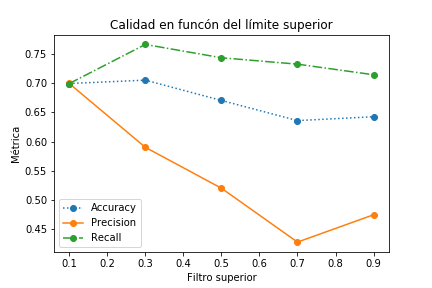
\includegraphics[width=84mm]{img/ul_calidad.png}}
\subfigure[]{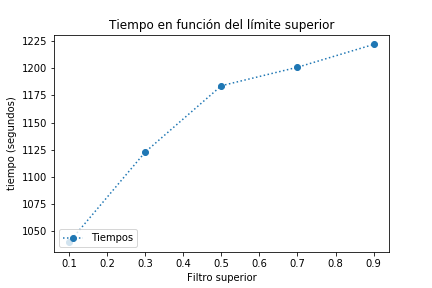
\includegraphics[width=84mm]{img/ul_tiempo.png}}
\caption{Calidad y tiempo en función del límite superior}
\label{fig:exp2-metricas-ul}
\end{figure}

De este prueba se desprende que la calidad del resultado tiende a disminuir a medida que se corre el límite superior. Al hacerlo se van incluyendo palabras muy comunes como features que no contribuyen a clasificar correctamente el sentimiento de una reseña ya que precisamente por el hecho de contar con una elevada frecuencia, aparecen en ambos tipos de reviews, sea estas positivas o negativas. \\

En cuanto al tiempo de computo requerido para procesar el método, este tienda a aumentar a la par del límite superior ya que se cuentan con más palabras de cada reseña con las cuales tomar la distancia en el algoritmo de KNN. \\


\begin{figure}[H]
\subfigure[]{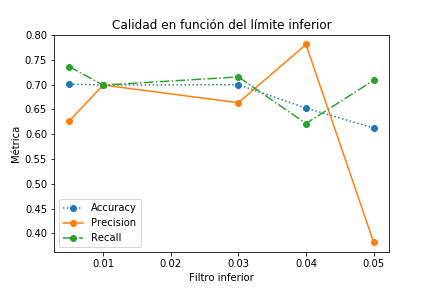
\includegraphics[width=84mm]{img/ll_calidad.png}}
\subfigure[]{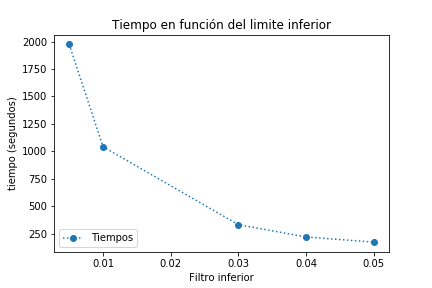
\includegraphics[width=84mm]{img/ll_tiempo.png}}
\caption{Calidad y tiempo del límite inferior}
\label{fig:exp2-metricas-ll}
\end{figure}

Por su parte, si fijamos el límite superior en 0.1 y variamos el inferior, vemos que la accuracy tiende a bajar a medida que que restringimos las palabras (es decir, aumentamos el límite inferior).\\
Estas palabras de un orden de magnitud menos frecuentes que las filtradas por el corrimiento del límite superior experimentado anteriormente pesan más en la discriminación del sentimiento de las reseñas. 
Creemos que esto se debe a que la menor frecuencia de las mismas redunda en una mayor relevancia como palabras descriptivas del carácter del texto analizado. \\

Así, una palabra que induce una aspecto negativo de una película no aparece en las reseñas con tanta frecuencia como un artículo o palabras neutrales, generalistas o propios del temática pero sin establecer una reacción a la misma (palabras como "film", "movies", "photography", "character", "protagonist", etc), pero deberían ser parte de la clase de reseñas que califican negativamente a la obra. Lo mismo sucede para las palabras que representan lo positivo. \\

Precision presenta un comportamiento más errático pero también tendiendo a la baja, mientras que recall se mantiene más constante. Al parecer si califica bien \\

El tiempo requerido para procesar los k vecinos más cercanos disminuye como se espera conforme aumentamos el límite inferior ya que descarta más features a considerar por el método. La diferencia notable entre 0.005 y 0.03 se debe a que en la primera la cantidad de palabras asciende a 2823 mientras que en la ultima solo se cuenta con 455. \\

Teniendo en cuenta esto, consideramos que tomando un límite inferior en 0.03 obtenemos una calidad de clasificación muy similar a 0.005 pero a mucho menor costo computacional. Con solo 455 palabras que se convierten en features logramos obtener una accuracy en torno a 0.75 y precision y recall de 0.71 y 0.65 respectivamente. \\
Por lo tanto nuestro filtrado de palabras para los posteriores experimentos es de 0.03 para el límite inferior y 0.1 para el superior. \\

\newpage
\subsection{Experimento 3: Normas métricas utilizadas en KNN}

Fijamos k en 20, sin pca, los límites del filtro como lo establecimos antes y variamos el k para ambas normas.\\

\begin{figure}[H]
\subfigure[]{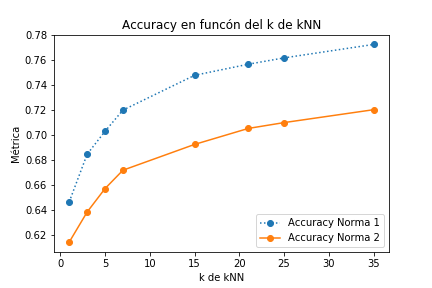
\includegraphics[width=84mm]{img/acc_normas.png}}
\subfigure[]{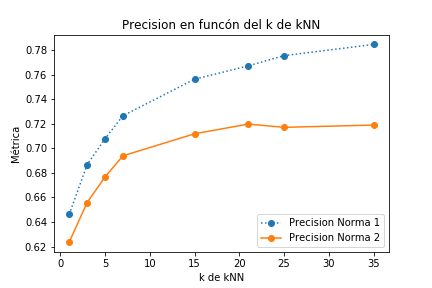
\includegraphics[width=84mm]{img/prec_normas.png}}
\subfigure[]{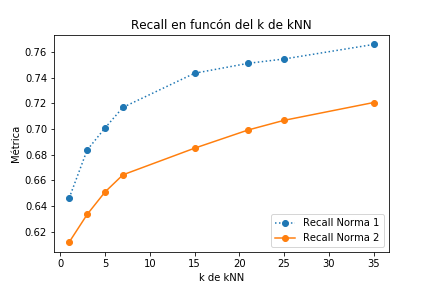
\includegraphics[width=84mm]{img/recall_normas.png}}
\caption{Calidad y tiempo de las normas en función del k de KNN}
\label{fig:exp3-calidad-normas}
\end{figure}

En las tres métricas para todos los k gana la norma Manhattan. La diferencia se vuelve mayor a mayor k.
Una posible explicación que le encontramos a este fenómeno es que los datos son palabras de un texto (una reseña de alguna película) y estas no pertenecen a una espacio físico como pueden ser las imágenes a reconocer (caras, dígitos, etc) donde la norma Euclídea parece ser una métrica más natural. \\
La norma Manhattan llega a un muy buen puntaje 0.78 en las tres métricas para k = 35. \\

\begin{figure}[H]
     \begin{center}
     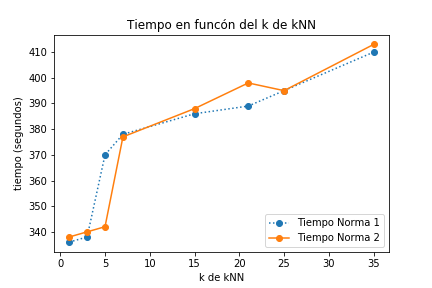
\includegraphics[width=100mm]{img/tiempo_normas.png} 
    \end{center}
\caption{Tiempo en función de k de KNN para ambas normas} \label{fig:exp3-tiempo-normas}
\end{figure}

Los tiempos son lógicamente muy similares ya que la norma 2 realiza algunas operaciones extras pero de complejidad constante y no cambia lo que demora asintóticamente el método de KNN en clasificar a las muestras de testing. \\

Teniendo en cuenta esto último y la diferencia de hasta un punto en todas las métricas para varios k, elegimos la norma Manhattan para los siguientes experimentos.

\newpage
\subsection{Experimento 4: k de KNN}

\begin{figure}[H]
\subfigure[]{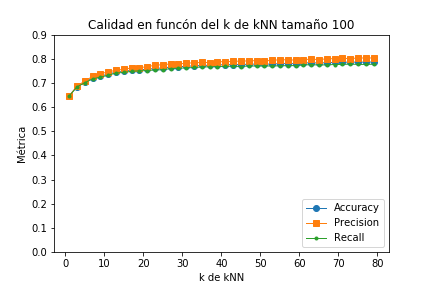
\includegraphics[width=84mm]{img/k_metricas_100.png}}
\subfigure[]{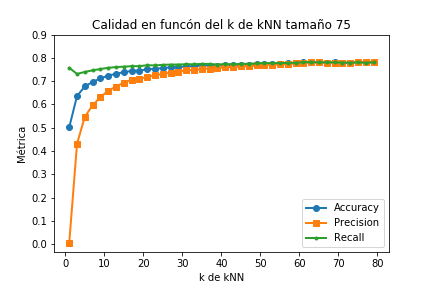
\includegraphics[width=84mm]{img/k_metricas_75.png}}
\subfigure[]{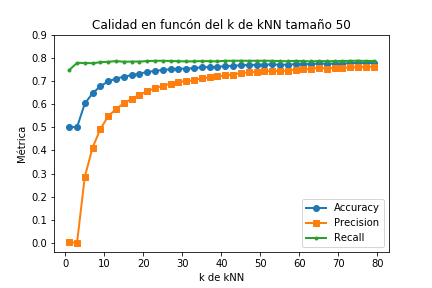
\includegraphics[width=84mm]{img/k_metricas_50.png}}
\subfigure[]{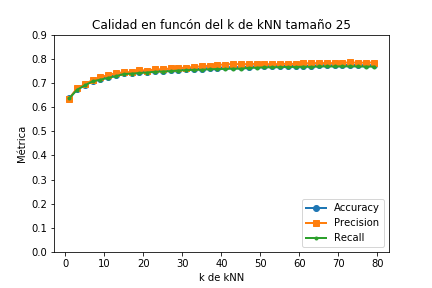
\includegraphics[width=84mm]{img/k_metricas_25.png}}
\caption{Calidad de k de KNN}
\label{fig:exp4-calidad-knn}
\end{figure}

Para el caso original (tamaño 100) se aprecia una mejora de 3 métricas de evaluación a la vez que se aumenta la cantidad de vecinos a considerar en el método de KNN. La mejora es más notable en los primeros 30 k. Luego parece converger con un accuracy de 0.78 en k = 79. \\

En nuestra opinión, el filtro de palabras utilizado juega un papel importante en este esquema, ya que como comentamos en dicho experimento, deja pocas palabras pero que seguramente son más descriptivas que las de muy baja frecuencia y las más comunes de mayor, frecuencia. En este balance, es posible que considerar una mayor cantidad de vecinos para determinar cuál es la clase mayoritaria entre estos sea la razón del aumento, aunque decreciente, de efectividad del algoritmo. \\

En los tamaños 75 y 50 se vislumbra un retraso en la convergencia. Hasta k = 20 las métricas son bastante peores que la del tamaño completo (especialmente la precisión) pero después se aproxima al mismo 0.78 para las tres. Esto puede deberse a que el menor tamaño dificulta la generalización del clasificador ya que no cuenta con tantas muestras como en el caso completo de 25000 casos de entrenamiento. \\
Sin embargo, con el 25$\%$ del dataset de entrenamiento ( 6250 muestras) se obtiene una curva de efectividad similar a la del tamaño completo pero de levemente menor puntaje (0.02 aproximadamente). No encontramos explicación para este caso. \\

\begin{figure}[H]
     \begin{center}
     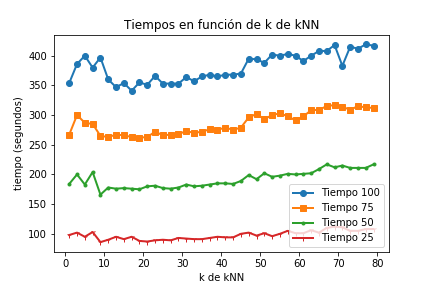
\includegraphics[width=100mm]{img/k_tiempos.png} 
    \end{center}
\caption{Tiempo en función de k de KNN para todos los tamaños} \label{fig:exp4-tiempo-knn}
\end{figure}

Tal como se esperaba, el tiempo no se ve afectado por el k escogido y tiende a ser constante en cada tamaño puesto que la única diferencia entre los k es obviamente la cantidad de vecinos a considerar, pero este costo es trivial en comparación con el de recorrer la matriz de de muestras y tomar la distancia entre ellas. \\
Por otra parte, el costo de un conjunto de entrenamiento de menor tamaño es menor a la de un conjunto de entrenamiento de mayor tamaño y así lo ilustra el gráfico. \\

Por todo lo discutido, tomamos k = 79 como una cantidad de vecinos razonables a considerar ya que tiende a converger a un puntaje ciertamente elevado en todas las métricas. En particular, se aproxima a 0.78 en accuracy, que es la métrica que más nos interesa puesto que distingue el sentimiento de una reseña. 
Además, no requiere de un costo computacional extra en comparación con menores k. \\


\newpage
\subsection{Experimento 5: $\alpha$ de PCA}

Se muestra como afecta el preprocesamiento de las muestras utilizando la técnica de Análisis de las Componentes Principales para la cantidad de vecinos más cercanos escogida en el experimento anterior pero también para los k = 1, 15 y 47.

En primer lugar, comparamos la accuracy, que entendemos que es la métrica más importante para el dominio del presente trabajo, obtenido al realizar PCA para distintos valores de $\alpha$ con la obtenida sin aplicar dicha técnica de selección de features. 

\begin{figure}[H]
\subfigure[]{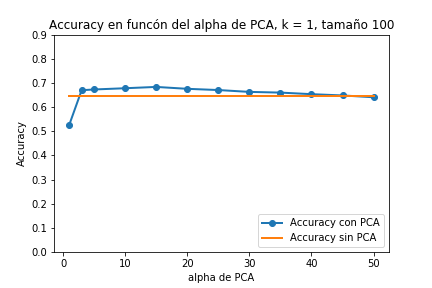
\includegraphics[width=84mm]{img/pca_acc_1_100.png}}
\subfigure[]{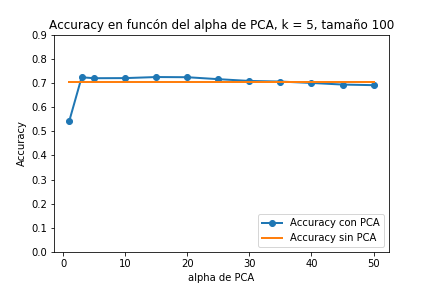
\includegraphics[width=84mm]{img/pca_acc_5_100.png}}
\subfigure[]{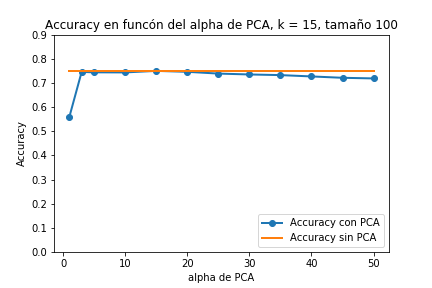
\includegraphics[width=84mm]{img/pca_acc_15_100.png}}
\subfigure[]{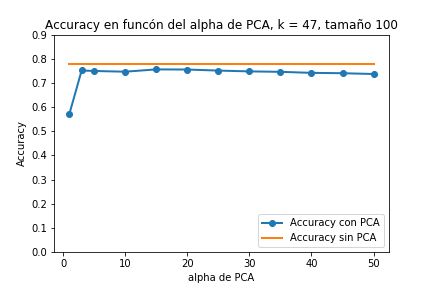
\includegraphics[width=84mm]{img/pca_acc_47_100.png}}
\subfigure[]{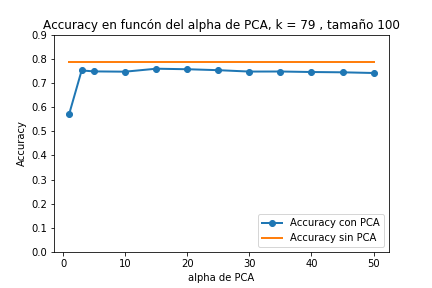
\includegraphics[width=84mm]{img/pca_acc_79_100.png}}
\caption{Accuracy en función de $\alpha$ de KNN+PCA para 5 k distintos. 
En una linea constante se muestra la accuracy para knn de ese k sin pca.}
\label{fig:exp5-acc-100}
\end{figure}

Observamos que para el método de k vecinos más cercanos con k = 1 ,k = 5, PCA mejora levemente los aciertos para $\alpha$ entre 2 y 30. Como esperábamos, el primer autovector no resulta suficiente para recrear los sentimientos pero a partir del segundo ya se cuenta con dos nuevos features construidos a partir de las 455 palabras que son más relevantes porque son los que más varían a lo largo del conjunto de entrenamiento y con ellos se logra superar al método kNN sin PCA.\\

Con dos componentes o características principales de las reseñas se descartan features no tan importantes de las 455 features/palabras filtradas que pueden generar ruido y se arman dos nuevos que discierne mejor si las reviews de películas son positivas o negativas. \\
La incorporación de componentes principales continua levemente incrementando la accuracy hasta $\alpha$ = 15 donde alcanza su máximo donde llega a superar por 0.05 puntos a la aplicación de kNN sin PCA, y comienza a revertir el puntaje conforme se agregan componentes principales. Esto último sucede en general para todos los k vecinos que se tomen y es un fenómeno que parece mostrar una de nuestras hipótesis.\\

Como intuimos en el planteamiento de esta prueba, un $\alpha$ demasiado grande (a partir del 20 según nuestro experimento para la base de datos analizada) produce una cantidad de autovectores que resulta ser no tan óptima puesto que se pierde información por la misma aplicación de la técnica de selección de features pero a su vez se toma una cantidad de componentes principales donde cada componente que se va agregando es menos relevante que el anterior y, dado que nuestro algoritmo de vecinos más cercanos no pondera features, estas nuevos autovectores solo contribuyen a disminuir la efectividad del método. \\

Para el k = 15, vemos como se emparda el uso de PCA con el knn sin en esto y los siguientes casos la no utilización del preprocesamiento siempre gana, con mayor diferencia para k = 79. 
Contrario a lo que pensábamos, no siempre es mejor realizar PCA.
A partir de un k suficientemente grande (mayor a 15), la cantidad de vecinos más cercanos a ser considerados en la votación del sentimiento mayoritario entre estos para determinar la clase a la que pertenece la muestra, compensa y supera en puntaje al empleo de la selección de features principales calculados a partir de las palabras cuyas frecuencias más difieren en las muestras del conjunto de entrenamiento.\\
De esta manera, el parámetro k, que define la cantidad de vecinos en orden ascendente de distancia a considerar en el cálculo de la clase mayoritaria a la que pertenece una muestra a ser testeada es más restrictivo y de mayor importancia que el $\alpha$ de PCA a la hora de analizar el sentimiento de una review. \\

En cuanto a las otras métricas, se obtuvo lo siguiente:

\begin{figure}[H]
\subfigure[]{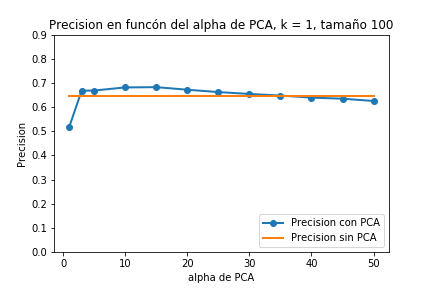
\includegraphics[width=84mm]{img/pca_prec_1_100.png}}
\subfigure[]{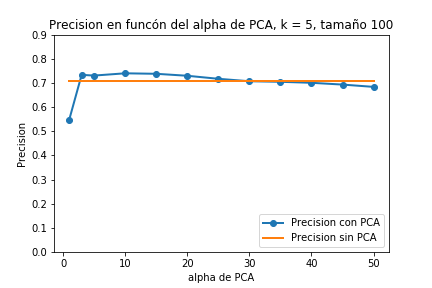
\includegraphics[width=84mm]{img/pca_prec_5_100.png}}
\subfigure[]{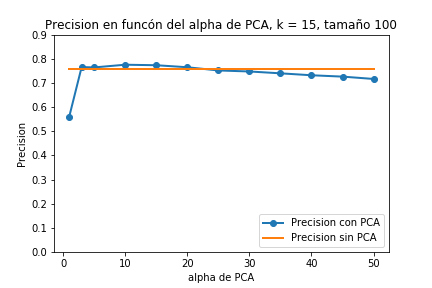
\includegraphics[width=84mm]{img/pca_prec_15_100.png}}
\subfigure[]{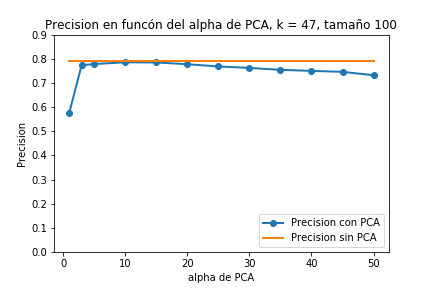
\includegraphics[width=84mm]{img/pca_prec_47_100.png}}
\subfigure[]{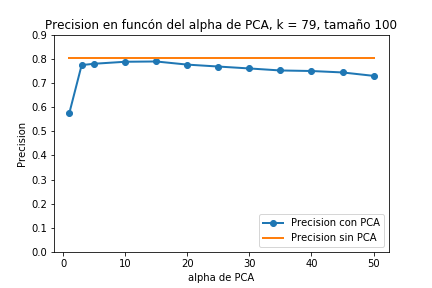
\includegraphics[width=84mm]{img/pca_prec_79_100.png}}
\caption{Precision en función de $\alpha$ de KNN+PCA para 5 k distintos. 
En una linea constante se muestra la precision para knn de ese k sin pca.}
\label{fig:exp5-prec-100}
\end{figure}

\begin{figure}[H]
\subfigure[]{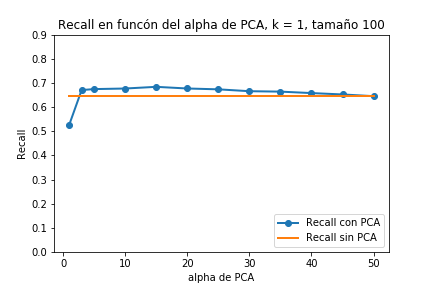
\includegraphics[width=84mm]{img/pca_recall_1_100.png}}
\subfigure[]{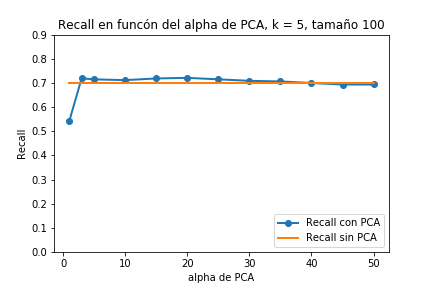
\includegraphics[width=84mm]{img/pca_recall_5_100.png}}
\subfigure[]{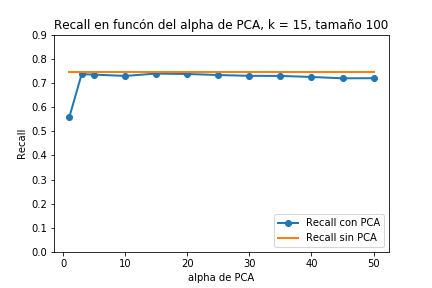
\includegraphics[width=84mm]{img/pca_recall_15_100.png}}
\subfigure[]{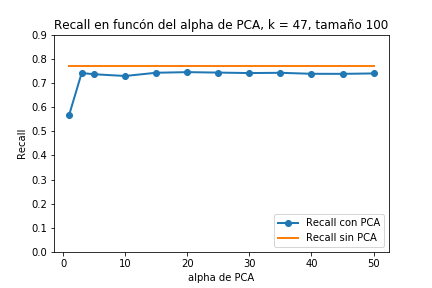
\includegraphics[width=84mm]{img/pca_recall_47_100.png}}
\subfigure[]{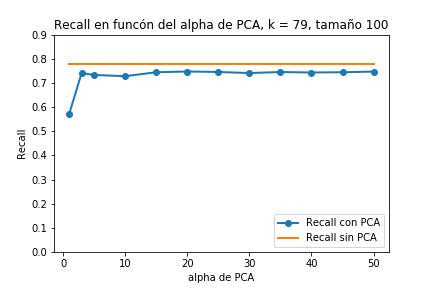
\includegraphics[width=84mm]{img/pca_recall_79_100.png}}
\caption{Recall en función de $\alpha$ de KNN+PCA para 5 k distintos. 
En una linea constante se muestra el recall para knn de ese k sin pca.}
\label{fig:exp5-recall-100}
\end{figure}

Se observa un patrón muy similar al caso de la accuracy. Para los k 1,5,15  PCA mejora la precision y el recall cuando se lo aplica con $\alpha$ entre 2 y 20 con respecto al kNN sin esta preprocesamiento.
Sin embargo, para k = 47 logra aproximadamente un empate y para k = 79 la precision y el recall son inferiores al kNN sin PCA. \\
A su vez, también se aprecia un patrón similar de caída o estancamiento de la efectividad lograda a medida que se incorporan más autovectores principales al cálculo. \\

Hasta aquí solo tomamos el tamaño completo del conjunto de entrenamiento. En los siguientes gráficos, se compara kNN + PCA para los distintos tamaños. Solo mostramos el caso sobre el k elegido (79). Para los otros k el resultado es similar. \\

\begin{figure}[H]
\subfigure[]{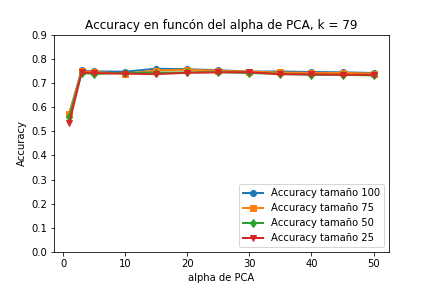
\includegraphics[width=84mm]{img/pca_tam_acc_79.png}}
\subfigure[]{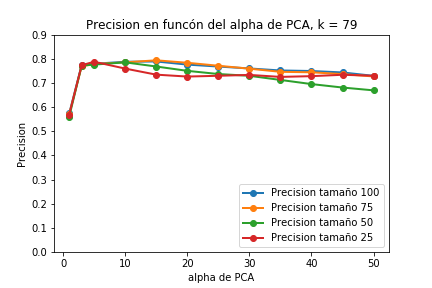
\includegraphics[width=84mm]{img/pca_tam_prec_79.png}}
\subfigure[]{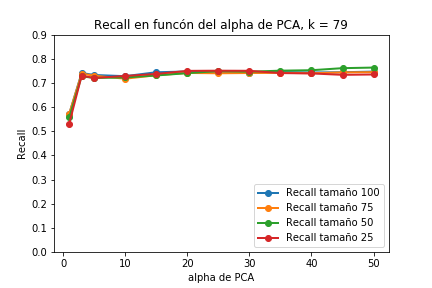
\includegraphics[width=84mm]{img/pca_tam_recall_79.png}}
\caption{Métricas en función de $\alpha$ de KNN+PCA para k = 79 y disintos 
tamaños del conjunto de entrenamiento.}
\label{fig:exp5-tam}
\end{figure}

De estas figuras se desprende que el tamaño es afectado de manera similar por $\alpha$ que al variar el k del experimento anterior. Conforme se disminuye el tamaño de del conjunto, decrece la accuracy del método. Al igual que en la variación de k, la diferencia no es elevada (solo 0.04 en promedio) pero y las de menor tamaño requieren de un $\alpha$ mayor para alcanzar su mejor performance de kNN + PCA. \\
En las demás métricas se mantiene un tendencia similar aunque con un leve aumento del recall para el tamaño 50.\\

De esta manera, la cantidad de muestras tomadas para entrenar al clasificador sigue pesando aún preprocesando dicho conjunto. A mayor tamaño mayor efectividad se logra dado que el método cuenta con un mayor número de reseñas para comparar y así generalizar el sentimiento de las mismas. \\

Por último, evaluamos el requerimiento temporal de computar PCA a medida que aumentamos la cantidad de componentes principales a considerar para k = 79 y tamaó 100: \\

\begin{figure}[H]
     \begin{center}
     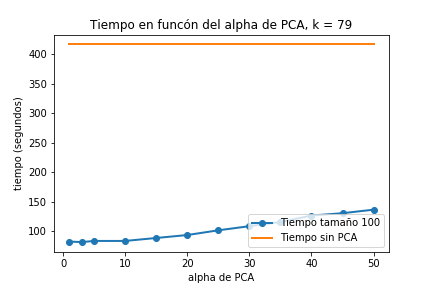
\includegraphics[width=100mm]{img/pca_tiempo_79_100.png} 
    \end{center}
\caption{Tiempo en función de $\alpha$ de PCA para k =79.} \label{fig:exp5-tiempo-knn}
\end{figure}

Lógicamente el cómputo de kNN+PCA aumenta si elegimos mayor cantidad de componentes principales ya que se debe realizar el método de la potencia $\alpha$ mientras se usa deflación sobre la matriz de Covarianza.\\

A su vez, kNN+PCA demora considerablemente menos en devolver una etiqueta que solo kNN. La razón por la cual acontece esto es que PCA se queda con pocos nuevos features, más precisamente $\alpha$ features, y por lo tanto la matriz que se utiliza en el kNN es de dimensión m muestras x $\alpha$ features, con $\alpha$ < 455 palabras. El costo de las iteraciones del método de la potencia no logran compensar mermar esta ganancia en tiempo de utilizar PCA , al menos para los primeros 50 $\alpha$. \\

Por lo tanto si no se necesita analizar el sentimiento de una reseña de manera casi instantánea o para un sistema en tiempo real, como creemos que ocurre en la mayoría de los casos donde se requiere clasificar este tipo de datos, kNN sin PCA con k = 79 obtiene mejores resultados en todas las métricas. \\
